% Created 2018-04-21 l� 22:33
\documentclass[11pt]{article}
\usepackage[utf8]{inputenc}
\usepackage[T1]{fontenc}
\usepackage{fixltx2e}
\usepackage{graphicx}
\usepackage{longtable}
\usepackage{float}
\usepackage{wrapfig}
\usepackage{rotating}
\usepackage[normalem]{ulem}
\usepackage{amsmath}
\usepackage{textcomp}
\usepackage{marvosym}
\usepackage{wasysym}
\usepackage{amssymb}
\usepackage{hyperref}
\tolerance=1000
\usepackage{color}
\usepackage{listings}
\author{Christian Zhuang-Qing Nielsen\thanks{201504624, christian@czn.dk}}
\date{\today}
\title{dOpt Compulsory Assignment 2 Re-handin}
\hypersetup{
  pdfkeywords={},
  pdfsubject={},
  pdfcreator={Emacs 25.1.1 (Org mode 8.2.10)}}
\begin{document}

\maketitle
\tableofcontents


\section{Show that the problem can be formulated as a maximum flow problem}
\label{sec-1}
The question of whether or not team 1 can win the championship can be formulated as a maximum flow problem. As we can assume without loss of generality that team 1 wins the remaining of their matches, we don't need to include them in our graph. Instead, we introduce a variable $g_i$ which is the maximum numbe of points team $i$ can receive if they win the remainder of their matches.

The network consists of a source node, a sink node, a node for every match and a node for every team. The source node sends two points to every match node, which them distributes them to one or both nodes of the teams linked to that specific match. The source node also sends the current points of each team to the team nodes. The team nodes then sends these as well as the points gained from the matches to the sink. If we specify the upper bound of $< p_1 + g_1$ we ensure that no team will exceed the maximum theoretical point of team one, and since we assume they team one wins all their games we now know that if the network is feasible, team one will win the championship. The network is shown below:

\begin{figure}[htb]
\centering
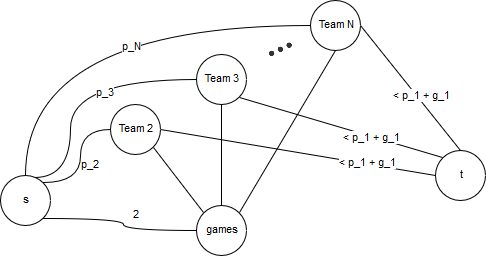
\includegraphics[width=.9\linewidth]{./network.png}
\caption{The illustrated network. In reality the games-node consists of a node for every match.o}
\end{figure}

\section{Why wouldn't the three-point rule work?}
\label{sec-2}
When utilising the two-point rule, there are in reality two cases: In the first case, one team wins and gains two points while the other gains none, and in the other case each team gains a point each (in case of a a draw). In both cases the amount of flow-units is exactly 2. This is not the case when using the three-point rule, as there are 3 flow-units in the winning case and only 2 in the draw-case. This makes the nodes in the network unbalanced, and thus it cannot be defined as a maximum-flow problem. Sending three flow-units to every match and redirecting the additional flow to the sink wouldn't work either, as it could result in the case where a team got two points somehow, which isn't using this rule.

\section{Formulate the problem (with three-point rule) as a integer LP problem}
\label{sec-3}
For every match $m^k_{ij}$, where $k$ is match number, $i$ is the team number of the first team and $j$ the number of the second team, we define it to be:
\begin{equation*}
$m^k_{ij} = x_{i}+y_{j}+z_{ij}$, \qquad where $i \neq j$ and $m^k_{ij} = 1$ for every $k$.
\end{equation}

The constraints on $m$ ensure that the same team cannot play itself, and that there are only a single outcome of every match (either team 1 wins, or team 2 wins, or they draw).

Furthermore, we define
\begin{equation*}
$h_{i} = 3*x'_i+3*y'_i+z'_i$
\end{equation}
As the number of points team $i$ has won from the remaining matches. To clairy, $x'_i$ is the number of times team $i$ has won in all $k$ matches as team 1. Similarly, $y'_i$ is the number of times team $i$ has won as the second team, and the final variable $z'_i$ is the number of times team $i$ has tied with other teams.

We now define a new variable $t_i$:
\begin{equation*}
$t_{i} = p_{i} + h_{i}$
\end{equation}
This variable is the total amount of points team $i$ has optained once all the remaining matches are played. We can now make a very important constraint (given we are asking the question of whether team $1$ can win):
\begin{equation*}
$t_i < t_1$, \qquad for $i=2, \dots , N$.
\end{equation} 
$t_1$ is a constant as we can assume they win all of their remaining matches. This ensures us, that to have a feasible program, all the other teams must not be able to exceed the amount of points team $1$ has at the end of the championship.

Finally we add the constraints that all variables are non-negative. For our objective function we minimise 0, as we only need to check if the program is feisible (and thus whether or not it is possible for team 1 to win the championship).
% Emacs 25.1.1 (Org mode 8.2.10)
\end{document}
